% This file was created with tikzplotlib v0.10.1.
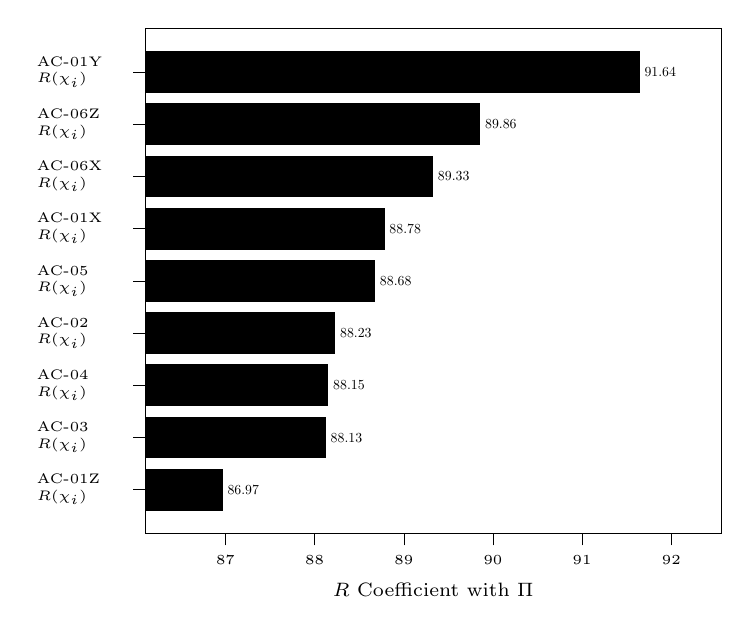
\begin{tikzpicture}

\definecolor{darkgray176}{RGB}{176,176,176}
\definecolor{sienna1279963}{RGB}{127,99,63}
\pgfplotsset{every tick label/.append style={font=\tiny}}

\begin{axis}[
tick align=outside,
tick pos=left,
x grid style={darkgray176},
xlabel={\scriptsize {$R$ Coefficient with $\boldsymbol{\Pi}$}},
xmin=86.0986827645007, xmax=92.5612231215855,
xtick style={color=black},
y grid style={darkgray176},
ymin=-0.84, ymax=8.84,
ytick style={color=black},
ytick = {0, 1, 2, 3, 4, 5, 6, 7, 8},
yticklabels= {
\parbox{11mm}{AC-01Z $\mathbb{R}(\boldsymbol{\chi_i})  $},
\parbox{11mm}{AC-03  $\mathbb{R}(\boldsymbol{\chi_i})  $}, 
\parbox{11mm}{AC-04  $\mathbb{R}(\boldsymbol{\chi_i})  $}, 
\parbox{11mm}{AC-02  $\mathbb{R}(\boldsymbol{\chi_i})  $}, 
\parbox{11mm}{AC-05  $\mathbb{R}(\boldsymbol{\chi_i})  $}, 
\parbox{11mm}{AC-01X $\mathbb{R}(\boldsymbol{\chi_i})  $}, 
\parbox{11mm}{AC-06X $\mathbb{R}(\boldsymbol{\chi_i})  $}, 
\parbox{11mm}{AC-06Z $\mathbb{R}(\boldsymbol{\chi_i})  $}, 
\parbox{11mm}{AC-01Y $\mathbb{R}(\boldsymbol{\chi_i})  $}, 
},
height=80mm,
width=89mm,
]
\draw[draw=none,fill=black] (axis cs:0,-0.4) rectangle (axis cs:86.9683664287886,0.4);
\draw[draw=none,fill=black] (axis cs:0,0.6) rectangle (axis cs:88.1251568666528,1.4);
\draw[draw=none,fill=black] (axis cs:0,1.6) rectangle (axis cs:88.1532240479358,2.4);
\draw[draw=none,fill=black] (axis cs:0,2.6) rectangle (axis cs:88.2312767527318,3.4);
\draw[draw=none,fill=black] (axis cs:0,3.6) rectangle (axis cs:88.6772687275304,4.4);
\draw[draw=none,fill=black] (axis cs:0,4.6) rectangle (axis cs:88.7845349607805,5.4);
\draw[draw=none,fill=black] (axis cs:0,5.6) rectangle (axis cs:89.3280103396995,6.4);
\draw[draw=none,fill=black] (axis cs:0,6.6) rectangle (axis cs:89.8571596447509,7.4);
\draw[draw=none,fill=black] (axis cs:0,7.6) rectangle (axis cs:91.6447753679064,8.4);
\draw (axis cs:86.9683664287886,0) ++(0pt,0pt) node[
  scale=0.5,
  anchor=west,
  text=black,
  rotate=0.0
]{86.97};
\draw (axis cs:88.1251568666528,1) ++(0pt,0pt) node[
  scale=0.5,
  anchor=west,
  text=black,
  rotate=0.0
]{88.13};
\draw (axis cs:88.1532240479358,2) ++(0pt,0pt) node[
  scale=0.5,
  anchor=west,
  text=black,
  rotate=0.0
]{88.15};
\draw (axis cs:88.2312767527318,3) ++(0pt,0pt) node[
  scale=0.5,
  anchor=west,
  text=black,
  rotate=0.0
]{88.23};
\draw (axis cs:88.6772687275304,4) ++(0pt,0pt) node[
  scale=0.5,
  anchor=west,
  text=black,
  rotate=0.0
]{88.68};
\draw (axis cs:88.7845349607805,5) ++(0pt,0pt) node[
  scale=0.5,
  anchor=west,
  text=black,
  rotate=0.0
]{88.78};
\draw (axis cs:89.3280103396995,6) ++(0pt,0pt) node[
  scale=0.5,
  anchor=west,
  text=black,
  rotate=0.0
]{89.33};
\draw (axis cs:89.8571596447509,7) ++(0pt,0pt) node[
  scale=0.5,
  anchor=west,
  text=black,
  rotate=0.0
]{89.86};
\draw (axis cs:91.6447753679064,8) ++(0pt,0pt) node[
  scale=0.5,
  anchor=west,
  text=black,
  rotate=0.0
]{91.64};

\end{axis}

\end{tikzpicture}
